%%
%% Copyright 2007, 2008, 2009 Elsevier Ltd
%%
%% This file is part of the 'Elsarticle Bundle'.
%% ---------------------------------------------
%%
%% It may be distributed under the conditions of the LaTeX Project Public
%% License, either version 1.2 of this license or (at your option) any
%% later version.  The latest version of this license is in
%%    http://www.latex-project.org/lppl.txt
%% and version 1.2 or later is part of all distributions of LaTeX
%% version 1999/12/01 or later.
%%
%% The list of all files belonging to the 'Elsarticle Bundle' is
%% given in the file `manifest.txt'.
%%

%% Template article for Elsevier's document class `elsarticle'
%% with numbered style bibliographic references
%% SP 2008/03/01
%%
%%
%%
%% $Id: elsarticle-template-num.tex 4 2009-10-24 08:22:58Z rishi $
%%
%%
\documentclass[preprint,12pt,3p]{elsarticle}

%% Use the option review to obtain double line spacing
%% \documentclass[preprint,review,12pt]{elsarticle}

%% Use the options 1p,twocolumn; 3p; 3p,twocolumn; 5p; or 5p,twocolumn
%% for a journal layout:
%% \documentclass[final,1p,times]{elsarticle}
%% \documentclass[final,1p,times,twocolumn]{elsarticle}
%% \documentclass[final,3p,times]{elsarticle}
%% \documentclass[final,3p,times,twocolumn]{elsarticle}
%% \documentclass[final,5p,times]{elsarticle}
%% \documentclass[final,5p,times,twocolumn]{elsarticle}

%% if you use PostScript figures in your article
%% use the graphics package for simple commands
%% \usepackage{graphics}
%% or use the graphicx package for more complicated commands
%% \usepackage{graphicx}
%% or use the epsfig package if you prefer to use the old commands
%% \usepackage{epsfig}

%% The amssymb package provides various useful mathematical symbols
\usepackage{amssymb}
\usepackage[ruled,vlined]{algorithm2e}
\usepackage{amsmath}
\usepackage{multirow}

%% The amsthm package provides extended theorem environments
%% \usepackage{amsthm}

%% The lineno packages adds line numbers. Start line numbering with
%% \begin{linenumbers}, end it with \end{linenumbers}. Or switch it on
%% for the whole article with \linenumbers after \end{frontmatter}.
%% \usepackage{lineno}

%% natbib.sty is loaded by default. However, natbib options can be
%% provided with \biboptions{...} command. Following options are
%% valid:

%%   round  -  round parentheses are used (default)
%%   square -  square brackets are used   [option]
%%   curly  -  curly braces are used      {option}
%%   angle  -  angle brackets are used    <option>
%%   semicolon  -  multiple citations separated by semi-colon
%%   colon  - same as semicolon, an earlier confusion
%%   comma  -  separated by comma
%%   numbers-  selects numerical citations
%%   super  -  numerical citations as superscripts
%%   sort   -  sorts multiple citations according to order in ref. list
%%   sort&compress   -  like sort, but also compresses numerical citations
%%   compress - compresses without sorting
%%
%% \biboptions{comma,round}

% \biboptions{}


\journal{Information Systems}

\begin{document}

\begin{frontmatter}

\title{Evaluation of different text representation techniques and distance metrics using KNN for documents classification}

\author[label1]{Luis-Alexander Calvo-Valverde}
\address[label1]{DOCINADE, Instituto Tecnol\'{o}gico de Costa Rica, Cartago, Costa Rica}
\ead{lcalvo@itcr.ac.cr}

\author[label2]{Jos\'{e}-Andr\'{e}s Mena-Arias}
\address[label2]{Maestr\'{i}a en Computaci\'{o}n, Instituto Tecnol\'{o}gico de Costa Rica}
\ead{andres.menaarias@gmail.com}


\begin{abstract}
Nowadays, text data is a fundamental part in databases around the world and one of the biggest challenges has been the extraction of meaningful information from large sets of text. This problem can be seen as a classification algorithms problem where text documents should be organized within categories. It also implies the problem of calculating how similar is a text value with respect to another. Existing literature about solving this kind of problems is extensive, however, during the last 25 years the statistical methods (where similarity functions are applied over vectors of words) have achieved good results in many areas of text mining. Additionally, topic modeling has arisen in the last years as a promising alternative to existing methods by achieving dimensional reduction and incorporating the semantic factor when classifying documents. This paper evaluates traditional data representation techniques and similarity metrics (Bags of Words, Cosine and Jaccard) respect to topic modeling techniques and probability distributions comparison (Latent Dirichlet Allocation and Kullback-Leibler Divergence). The results show that the accuracy scores achieved by using document representations obtained thought Latent Dirichlet Allocation, combined with the relative entropy metric, were similar to the ones obtained by using traditional text classification techniques. The topics modeling manages to abstract thousands of words in less than 60 topics for the main set of experiments. The results also highlight cons, improvement areas and potential scenarios where such models could achieve a better performance. 
\end{abstract}

\begin{keyword}
%% keywords here, in the form: keyword \sep keyword
text similarity \sep text classification \sep KNN \sep topic modeling 
%% MSC codes here, in the form: \MSC code \sep code
%% or \MSC[2008] code \sep code (2000 is the default)
\end{keyword}

\end{frontmatter}

%%
%% Start line numbering here if you want
%%
% \linenumbers

%% main text

\section{Introduction}
\label{introduction}


Nowadays, large volumes of text information are available on the Internet and in institutional databases with a clear trend of continuous growing, hence applying data mining and machine learning techniques over text data is becoming extremely relevant \cite{srivastava2009text}. One of the biggest challenges in this area has been the ability to extract meaningful information from large sets of text.\par

For example, consider those systems used in most of the companies to track application failures reported by users. Every time an user reports an issue, the support person receives certain information, including a free text description of the problem observed by the user. Once the support specialist takes action and resolves the issue, the system generally allows to take notes about the investigation done, the explanation of what caused the failure and select the root cause category from a dropdown. Suppose that someone wants to analyze the roots causes of issues received in the last year, but it is found that, in many cases, the category was not selected when the problem was resolved, causing the report to have missing values in multiple records. In this situation, the root cause categories could be estimated by analyzing the free text in the respective descriptions and notes taken for the issue. Even though this task could be done by people, when there are thousands of records in the database then there is a need of evaluating automated solutions where a program is able to find those relations between the text and the missing category.\par

Under this context, this paper analyses the problem of text classification, where an algorithm classifies the observed text values within different categories. Existing literature proposes different machine learning and data mining algorithms to solve classification problems in a supervised way \cite{tran2015multiple,truong2004learning, ishioka2014investigations}. Algorithms such as K-Nearest-Neighbors (KNN), where text distance metrics can be used to classify elements, are relevant for documents classification problems \cite{terzi2014text}.\par

Current literature about metrics to determine how similar is a text document with respect to another is very extensive. Statistical methods intend to create mathematical data representations of text without considering semantic nor linguistic properties and have shown very good results in the last 25 years in text mining areas \cite{srivastava2009text}. Statistic methods include the representation of documents through bags of words and the use of distance metrics such as Cosine and Jaccard \cite{wang2016non, soto2015similarity}. \par

Additionally, topic modelling has arisen as a promising alternative to the existing methods, by achieving good results in documents classification using probability distributions similarity, dimensional reduction and incorporating topics semantic \cite{ bae2014computing, bougiatiotis2016content, huang2008similarity, metzler2007similarity}. Latent Dirichlet Allocation (LDA) is one of the most popular techniques in this area, using both unsupervised and supervised learning \cite{mcauliffe2008supervised}. \par

This paper is focused on the evaluation of traditional data representation techniques and text distance metrics (bag of words, Cosine, Jaccard), respect to methods involving topic modelling and probability distributions comparison such as LDA and Kullback-Leibler divergence (KLD, also known as relative entropy). For that purpose, we analyze the results obtained after running several experiments using the techniques already mentioned to classify datasets of text documents. The results show that the accuracy scores achieved by using document representations obtained thought LDA, combined with the relative entropy metric, were similar to the ones obtained by using traditional text classification techniques. The topics modeling manages to abstract thousands of words in less than 60 topics for the main set of experiments. An additional analysis highlights cons, improvement areas and potential scenarios where such models could achieve a better performance. \par

The rest of the document is organized as follows. Section 2 summarizes the previous work done around text classification. In section 3 we describe the models theoretically. The details about the experiments are shown in section 4 and the obtained results are analyzed in section 5. Finally, in sections 6 and 7 we propose the future work and present the conclusions.

\section{Related work}
\label{related_work}

There has been a lot of work around algorithms to solve the problem of text classification in the areas of machine learning and data mining. This paper was focused on those methods aimed to find relationships among text and categorical attributes. In this section we summarize the work done by different authors about these topics.\par

In \cite{tran2015multiple,truong2004learning, ishioka2014investigations} several algorithms of supervised classification are considered, such as Hotdeck, KNN and Random Forest. These methods require a labeled training set of data and they use similarity metrics to define the relations among the elements to classify. There are other algorithms based on statistical models, such as Likelihood classification which uses Expectation-Maximization \cite{anagnostopoulos2014scaling} and Bayesian models (Naive Bayes and Bayesian Linear Regression) \cite{mavai2014survey}. Other popular techniques include mathematical models to approximate values and reduce errors based on training data, for example, Artificial Neural Networks \cite{nelwamondo2007missing} and Support Vector Machines \cite{hsu2003practical}. From all these algorithms, we considered the first group for this work since they were the best match for our problem by allowing the definition of similarity metrics.\par

When studying the classification of text documents, current literature is focused on two types of methods: linguistic and statistical \cite{srivastava2009text}. In linguistic methods, text is handled based on the processing of natural language, considering semantic representations and relationships of words within a linguistic model \cite{srivastava2009text}. Different authors have Incorporated semantics when comparing text documents, requiring the integration of external sources of knowledge and lexical data bases such as Wikipedia \cite{seifzadeh2015short} or WordNet  \cite{lazar2014improving, devraj2015twitter, martinez2014analysis}. In such methods, words similarity is determined by the degree of overlapping in their meanings or by the distance between two terms if represented using a graph of hyperonyms \cite{ devraj2015twitter}. Even though linguistic methods can achieve more expressive representations of text, they can also add more complexity due to the construction of semantic models and context-specific dependency in the data \cite{srivastava2009text}. This work made use of statistical methods which involve the mathematical representation of text without considering semantics or linguistic properties \cite{srivastava2009text}. The general process in statistic methods consist on using some technique to create a representation of documents and then to apply a function on these representations to calculate how similar are from each other. \par

The bag of words is the data representation technique used in most of the consulted literature \cite{aggarwal2015data,soto2015similarity,kumaran2004text,xu2012combining,srivastava2009text, lazar2014improving}. It consists on representing each text document as a vector of frequencies \cite{aggarwal2015data}. A variant of this representation uses Term Frequency-Inverse Document Frequency (TF-IDF) weighting \cite{araki2014annotation,soto2015similarity} where each word in a document is assigned a weight depending on their frequencies within an specific document and throughout all the documents.\par

The topic modelling technique known as LDA is used in \cite{lazar2014improving,bae2014computing} and considers two main concepts: 1) a single document can have several latent topics and 2) each topic can be drawn as a probability distribution of words (documents are represented as vectors of topics instead of bags of words). A supervised variant of LDA (sLDA) is proposed in \cite{mcauliffe2008supervised}, which incorporates a response variable (or class) when calculating the model of topics. That work uses sLDA to predict movies and web sites ratings based on the text of user reviews. Another research uses sLDA to classify and label images, representing each picture as a text document of keywords \cite{chong2009simultaneous}.\par

Regarding text distance metrics the literature is very extensive, being the Cosine similarity one of the most used techniques, like in \cite{liebman2016capturing,soto2015similarity}. Authors in \cite{bae2014computing} combine LDA representation with the Cosine function to calculate similarity among publications using the text of the title, abstract and author names. Other metrics used for both classification and grouping of text documents include the Jaccard similarity \cite{liebman2016capturing,soto2015similarity} and string comparison metrics like Levenshtein distance \cite{gong2009matching, treeratpituk2012name} and Longest Common Subsequence score \cite{islam2008semantic, soto2015similarity}.\par

Huang \cite{huang2008similarity} uses KLD to determine the distance between two documents, assuming probability distribution representations of the text. Results in \cite{huang2008similarity, metzler2007similarity} show that KLD outperforms Cosine, Jaccard and Euclidean distances when calculating the purity and the entropy on certain types of text datasets.\par

\section{Model descriptions}
\label{model_descriptions}

\subsection{KNN classification algorithm}

In this paper, we use KNN because it is a supervised classifier and can be configured to use text distance metrics as explained in a later section. KNN is an algorithm that selects the nearest ${k}$ observations to a certain value according to a distance metric. Even though it is categorized as a machine learning algorithm, KNN is sometimes called a lazy learner because it doesn't do a proper learning process and, instead, it uses the whole training dataset to classify an element \cite{mavai2014survey}.\par

Algorithm \ref{alg-KNN} shows the general idea of KNN used for text classification. The algorithm receives a training dataset $E$ and a test dataset $X$. The $FindNeighbors$ function returns a list of $k$ rows taken from $E$ where the values of the textual attributes are the nearest ones respect to the values of the same attributes in $X$ according to a distance function. The function $GetCategoryByVoting$ obtains the most frequent value in a categorical attribute from the rows stored in $neighbors$.\par

\begin{algorithm}
\label{alg-KNN}
\KwIn{k;E;X}
Let \textit{E} be a set of text documents labeled with a categorical attribute (training dataset)\;
Let \textit{X} be a set of text documents with no category associated\;
\ForEach{row \textit{x} in \textit{X}}{
	$neighbors\leftarrow$ FindNeighbors($k,x,E$)\;
	$category\leftarrow$ GetCategoryByVoting($neighbors$)\;
	$x[category] \leftarrow category$\;
}
\caption{KNN algorithm for text classification}
\end{algorithm}

\subsection{Documents representation using bag of words}

Let $D$ be a dataset composed by $m$ text documents where there is a total of $n$ different words. The main idea of a bag of words is to represent each document as a vector ${d=p_1,p_2,...,p_n}$, where the element $p_i$ corresponds to the frequency of the $i$-th word in that document \cite{srivastava2009text}. In this case, a set of documents can be seen as the matrix in equation \ref{equation_D}, being each ${p_{ij}}$ the value of the frequency of term $j$ in document $i$.

\begin{equation}
\label{equation_D}
D=\begin{pmatrix}
p_{11} & p_{12} & \cdots & p_{1n}\\ 
p_{21} & p_{22} & \cdots & p_{2n}\\ 
\vdots  & \vdots & \ddots  & \vdots \\ 
p_{m1} & p_{m2} & \cdots  & p_{mn}
\end{pmatrix}
\end{equation}

The vector representation of a document can also include a weight value instead of the frequency value. The technique Term Frequency - Inverse Document Frequency (TF-IDF) consists on calculating a weight for each word, combining the frequency of a term in a document and the number of documents containing such term respect to the total of documents \cite{srivastava2009text}. TF-IDF intends to highlight those terms that represent better specific documents and to lower the weight to irrelevant terms \cite{srivastava2009text}.\par

Other techniques commonly applied at the moment of creating bags of words include the removal of stop words (non relevant terms such as articles or pronouns), and word stemming (keeping only the root of words in order to create semantic grouping) \cite{srivastava2009text}.


\subsection{Text distance metrics}

In this paper we focused on evaluating term-based distance metrics, on which a text string is divided in terms, like in a bag of words, and this representation is used to do comparisons among vectors \cite{wang2016non}. A classification algorithm can use this metrics to calculate the distance between two elements.\par

Among the most common metrics used for words vector comparison are the Cosine and Jaccard similarities \cite{soto2015similarity,wang2016non}. However, there are some approaches based on probabilistic concepts that have also been used for text documents comparison, such as KLD \cite{bae2014computing,metzler2007similarity}. All these methods are explained in the below sections.

\subsubsection{Cosine distance}
This distance measures the degree of similarity between two documents ${d_{1}}$ and ${d_{2}}$ using the cosine of the angle formed by their vector representations \cite{soto2015similarity}, like shown in formula \ref{equation_cosine}.

\begin{equation}
\label{equation_cosine}
cos(\vec{d}_{1},\vec{d}_{2})=\frac{\vec{d}_{1}\cdot\vec{d}_{2}}{\parallel \vec{d}_{1}\parallel \parallel \vec{d}_{2} \parallel }
\end{equation}

\subsubsection{Jaccard similarity}
Having two bags of words ${d_{1}}$ and ${d_{2}}$ as two sets of elements (without considering terms frequency), the Jaccard similarity is defined in equation \ref{equation_jaccard} as the size of the intersection of ${d_{1}}$ and ${d_{2}}$ divided by the size of the union of the same sets \cite{aggarwal2015data}.

\begin{equation}
\label{equation_jaccard}
jaccard(\vec{d}_{1},\vec{d}_{2}) = \frac{\mid \vec{d}_{1}\cap \vec{d}_{2}\mid}{\mid\vec{d}_{1}\cup \vec{d}_{2}\mid}
\end{equation}

\subsubsection{Kullback-Leibler divergence}

Considering a document as a probability distribution of words represented in a vector, we can use KLD to measure the level of entropy between two probability distributions \cite{huang2008similarity}. So if n is the total of words in a collection of documents, two documents ${d_{1}}$ and ${d_{2}}$ can be represented as probability distributions ${\vec{d_{i}}=p_{i,1}, p_{i,2},…, p_{i,n}}$ where the value of ${p_{i,j}}$ represents the probability of word $j$ belonging to document ${d_{i}}$ for ${i \in \left \{ 1,2 \right \}}$ and ${1 \leq  j \leq  n}$, then KLD is calculated as shown in equation \ref{equation_KL}.
\begin{equation}
\label{equation_KL}
D_{KL}(\vec{d_{1}}\parallel\vec{d_{2}})=\sum_{j=1}^{n}{p_{1,j}\times log(\frac{p_{1,j}}{p_{2,j}})}
\end{equation}

KLD has been used in documents clustering and it is not symmetric, hence it should be combined with other methods to get a single value, such a weighted average \cite{huang2008similarity}.\par

\subsection{Topics modelling}

Topic modelling has arisen as a robust technique to structure collections of documents by using probabilistic models to find hidden semantic patterns \cite{srivastava2009text}. it represents an alternative method to achieve dimensional reduction and it has several advantages compared to other models of semantic analysis \cite{aggarwal2015data}.\par

This work used the documents representations with topics obtained through LDA, which is explained in the next section.

\subsubsection{Latent Dirichlet Allocation}

LDA is a probabilistic model used to classify documents in topics considering two aspects: 1) the same document can have several latent topics and 2) each topic can be represented a distribution of words \cite{bae2014computing}. In this case, a documents will be assigned probabilities of latent topics where, at the same time, each topic is a probability distribution of words.\par

The idea of LDA is to achieve dimensional reduction (compared to traditional representations using bag of words) and easily assign probabilities to new documents that were not part of the training dataset \cite{aggarwal2015data}.\par

Even though LDA was originally created to discover latent topics in an unsupervised way \cite{blei2003latent}, this paper explores the supervised variant proposed in \cite{mcauliffe2008supervised}. In supervised LDA, if we have $K$ topics, ${\beta_{1:K}}$ (where each ${\beta_{k}}$ is a vector of probabilities distribution per topic), a Dirichlet parameter ${\alpha}$, and parameters $\eta$ and $\sigma^{2}$ of the response variable \cite{mcauliffe2008supervised}. It is assumed that each text document is generated as follows:

\begin{enumerate}
   \item Get topic proportions ${\theta \mid \alpha \sim Dir(\alpha)}$.
   \item For each word:
   \begin{itemize}
     \item Assign a topic ${z_n \mid \theta \sim Mult(\theta)}$.
     \item Get a word ${w_n \mid z_n,\beta_{1:k}  \sim Mult(\beta_{z_n})}$.
   \end{itemize}
   \item Get response variable (class) ${y \mid z_{1:N},\eta,\sigma^{2}  \sim N(\eta^{T}\bar{z},\sigma^{2})}$.
\end{enumerate} 

This generative model can be observed in figure \ref{figure-sLDA}. Each node denotes a random variable, while edges represent dependencies. Boxes denote repetition for $D$ documents, $K$ topics y $N$ words \cite{srivastava2009text}.

\begin{figure}[h]
\caption{Graphical representation of supervised LDA \cite{mcauliffe2008supervised}.}
\label{figure-sLDA}
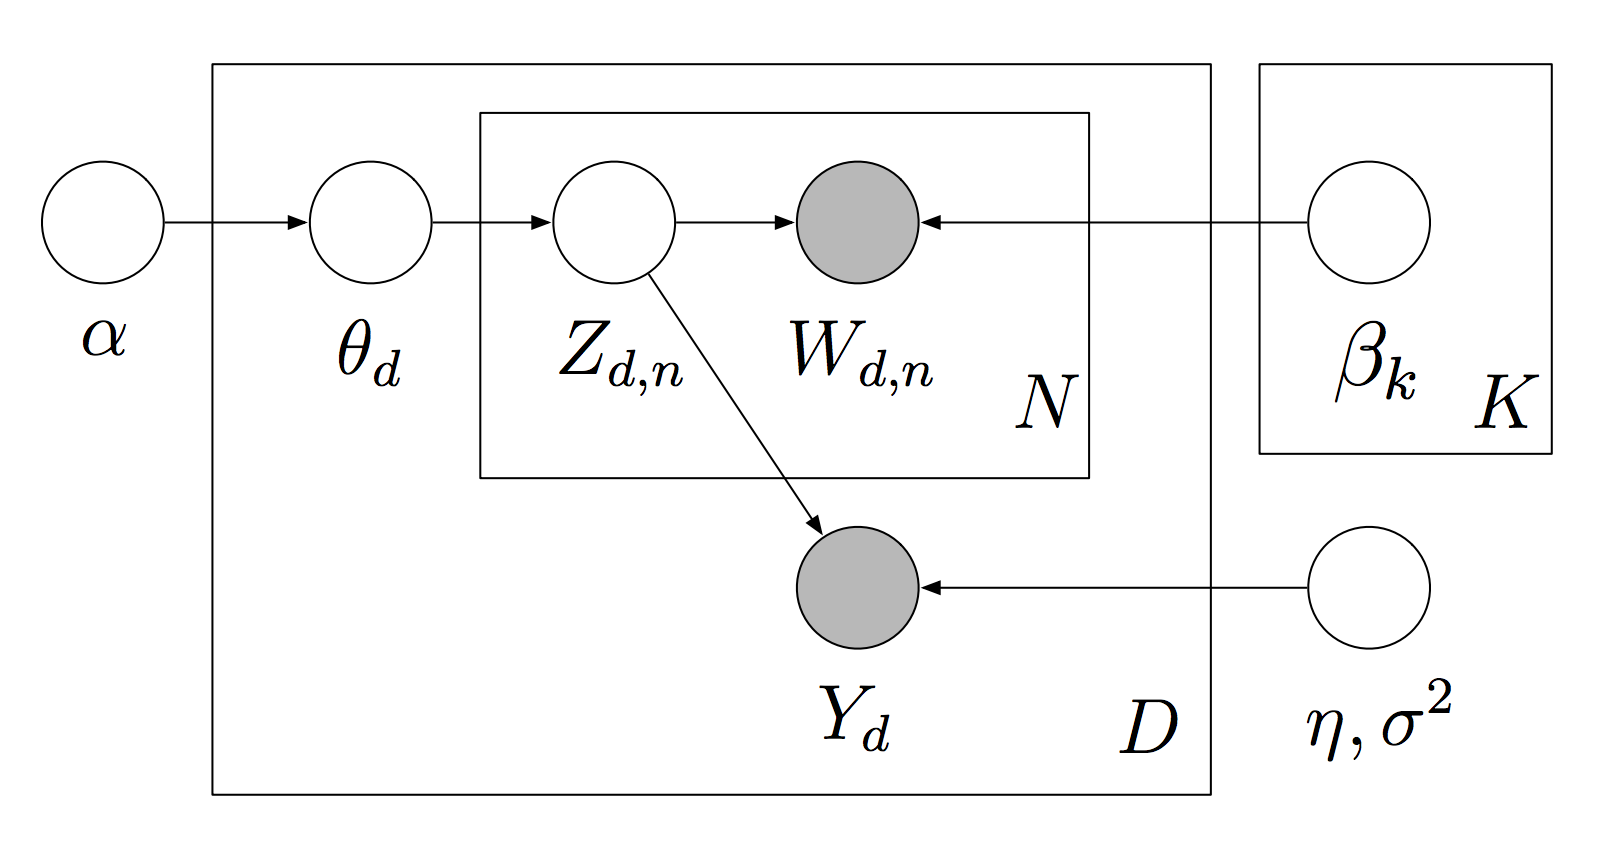
\includegraphics[width=\textwidth]{sLDA}
\end{figure}

In LDA, the final representation of a document ${d_{i}}$ is not a bag of words, but a vector of $k$ latent topics ${\vec{d_{i}}=p_{i,1}, p_{i,2},…, p_{i,k}}$ where the value of ${p_{i,j}}$ represents the probability that ${d_{i}}$ belongs to topic $j$ for ${1 \leq  j \leq  n}$ \cite{ bae2014computing, aggarwal2015data}. Subsequently, the similarity between two probability distributions can be calculated using a similarity metric. This paper was focused on the vector representation of documents only and not the complete LDA algorithm nor its prediction model.


\section{Experimental setup}
\label{experimental_setup}

\subsection{Development environment}

Experiments were executed on a virtual server with two processors of 2GHz each and 4GB of RAM running Ubuntu 16.04 distribution.\par
Documents representation as vectors of words were done using package RTextTools 1.4.2 in R version 3.2.3, while the main algorithms (KNN and text distance metrics) were implemented in Python version 3.5.2 using scikit-learn 0.18 libraries.\par
For supervised LDA, we used the C++ implementation based on the work of \cite{mcauliffe2008supervised,chong2009simultaneous} and published in the author's website \footnote{https://github.com/blei-lab/class-slda}.

\subsection{Datasets}

The data used in this experiments was extracted from the Reuters collection for text classification obtained from the UCI public repository \footnote{http://archive.ics.uci.edu/ml/datasets/Reuters-21578+Text+Categorization+Collection}.\par

To simplify the execution of experiments, we created two datasets by transforming and compiling a subset of the XML files taken from Reuters collection. We named these datasets reuters-1 and reuters-2:

\begin{itemize}
\item \textbf{reuters-1}. Contains two attributes: text and category. Each category value can be one of the 44 topics defined in the original Reuters dataset.
\item \textbf{reuters-2}. It also contains two attributes: text and category. In this case, each category value can be one of the 59 places defined in the original Reuters dataset.
\end{itemize}

\subsection{Implementation of data representation techniques}

The bags of words were generated from the original text documents using RTextTools package. We also applied removal of stop words and words stemming. Each file was transformed into two representations, one containing term frequencies and another using TF-IDF representation. For reuters-1 the bags of words consisted on matrices of 1063 documents by 6444 words, while for reuters-2 the dimension of the matrices was of 1641 documents by 8666 words.\par

To generate the vectors of topics, we used the C++ implementation of supervised LDA. The code was modified to allow us the extraction of the topic models representations. Even though the complete LDA algorithm does both estimation and inference operations, for this work we just needed the vectors of topics representations generated in the estimation step. The resulted LDA representations consisted on a matrix of 1063 documents by 44 topics for reuters-1, and a matrix of 1641 documents by 59 topics for reuters-2.\par

At this point we also partitioned the data representations in a set of 25\% test data and a set of 75\% training data. This allowed to execute all the experiments under the same conditions (same training and test data for all the experiments).

\subsection{Implementation of KNN and the text distance metrics}

KNN algorithm was implemented using the module KNeighborsClassifier from sklearn Python package. This module can be configured with customized similarity functions, which allowed us to define and incorporate the text distance metrics desired. We used Jaccard and Cosine implementations included within the sklearn package and for KLD we used the entropy metric from scipy package.

\subsection{Parameters selection}

The main parameter for KNN is the value of $k$ which determines the number of neighbors to consider when labeling a document. To select this parameter, we executed a subset of the experiments using multiple $k$ values and calculated the accuracy obtained on each case. We observed that the accuracy tended to decrease as we increased the value of $k$, and for such reason we used ${k=1}$ and ${k=11}$ to run the full set of experiments and analyze the results.\par

In the case of supervised LDA, we fixed the number of iterations and the error convergence thresholds with the library default values to simplify the selection and avoid performance issues (execution time increased considerably when slightly increasing the default values). Given the variety of text documents, we considered using three different values of $\alpha$: 0.2 (assumes text documents very different from each other and with few topics), 0.8 (assumes similar text documents with many topics each) and an intermediate value of 0.5. And finally, the number of topics was defined based on each dataset, assuming that the number of topics can be similar to the number of different classes (44 topics for reuters-1 and 59 topics for reuters-2).


\section{Results and analysis}
\label{results_and_analysis}

The results are shown in table \ref{table-results}, which contains the accuracy, precision, recall and F1 score obtained on each experiment for the two datasets. Each experiment involved a data representation technique, a text distance metric and the KNN algorithm. Data represented as bags of words was divided in two groups: with TF-IDF and without TF-IDF, while LDA representations were divided in three groups based on the different values of $\alpha$. Al the scores in the table were calculated using the macro-weighted metrics defined in the sklearn package. On this work we focused on the accuracy and the F1 score for the analysis.

\begin{table}[h]
\centering
\caption{Results for each experiment per dataset, value of $k$ and representation-metric combination. The best scores are highlighted for each set of experiments using the same dataset and value of $k$.}
\label{table-results}
{\tiny
\begin{tabular}{|l|l|l|l|l|l|l|}
\hline
 
{ \textbf{Dataset}}                 & { \textbf{k}} & { \textbf{Representation / Metric}}                           & { \textbf{Accuracy}} & { \textbf{Precision}} & { \textbf{Recall}} & { \textbf{F1}}       \\ \hline
 
\multirow{18}{*}{ \textbf{reuters-1}}                     & \multirow{9}{*}{ 1}         & LDA $\alpha$=0.2 / Cosine                                                              & { 0.8}                & { 0.804452}           & { 0.8}                   & { 0.792715}          \\ \cline{3-7}
					                  &                             & LDA $\alpha$=0.5 / Cosine                                                              & { 0.8}                & { 0.821869}           & { 0.8}                   & { 0.803953}          \\ \cline{3-7}
 
					                  &                             & LDA $\alpha$=0.8 / Cosine                                                              & { 0.816}              & { 0.815385}           & { 0.816}                 & { 0.811214}          \\ \cline{3-7}
					                  &                             & LDA $\alpha$=0.2 / KLD                                                      & { 0.8}                & { 0.797469}           & { 0.8}                   & { 0.789491}          \\ \cline{3-7}
 
					                  &                             & LDA $\alpha$=0.5 / KLD                                                      & { 0.768}              & { 0.776959}           & { 0.768}                 & { 0.759982}          \\ \cline{3-7}
					                  &                             & LDA $\alpha$=0.8 / KLD                                                      & { 0.8}                & { 0.797469}           & { 0.8}                   & { 0.789491}          \\ \cline{3-7}
 
					                  &                             & \begin{tabular}[c]{@{}l@{}}Bag of words with TF-IDF / \\ Cosine\end{tabular}  & { 0.808}              & { 0.834513}           & { 0.808}                 & { 0.808946}          \\ \cline{3-7}
					                  &                             & \begin{tabular}[c]{@{}l@{}}Bag of words without TF-IDF / \\ Cosine\end{tabular}  & { 0.856}              & { 0.860481}           & { 0.856}                 & { 0.852386}          \\ \cline{3-7}
 
					                  &                             & \begin{tabular}[c]{@{}l@{}}Bag of words without TF-IDF / \\ Jaccard\end{tabular} & { \textbf{0.9}}       & { \textbf{0.900628}}  & { \textbf{0.9}}          & { \textbf{0.893534}} \\ \cline{2-7}
					                  & \multirow{9}{*}{ 11}        & LDA $\alpha$=0.2 / Cosine                                                              & { 0.796}              & { 0.779623}           & { 0.796}                 & { 0.780964}          \\ \cline{3-7}
 
                					  &                             & LDA $\alpha$=0.5 / Cosine                                                              & { 0.788}              & { 0.754407}           & { 0.788}                 & { 0.762225}          \\ \cline{3-7}
					                  &                             & LDA $\alpha$=0.8 / Cosine                                                              & { 0.78}               & { 0.758448}           & { 0.78}                  & { 0.757489}          \\ \cline{3-7}
 
					                  &                             & LDA $\alpha$=0.2 / KLD                                                      & { 0.828}              & { 0.796299}           & { 0.828}                 & { 0.808493}          \\ \cline{3-7}
					                  &                             & LDA $\alpha$=0.5 / KLD                                                      & { 0.824}              & { 0.797579}           & { 0.824}                 & { 0.798982}          \\ \cline{3-7}
 
					                  &                             & LDA $\alpha$=0.8 / KLD                                                      & { 0.804}              & { 0.760077}           & { 0.804}                 & { 0.773005}          \\ \cline{3-7}
					                  &                             & \begin{tabular}[c]{@{}l@{}}Bag of words with TF-IDF / \\ Cosine\end{tabular}  & { 0.816}              & { 0.803179}           & { 0.816}                 & { 0.797044}          \\ \cline{3-7}
 
					                  &                             & \begin{tabular}[c]{@{}l@{}}Bag of words without TF-IDF / \\ Cosine\end{tabular}  & { 0.844}              & { 0.807863}           & { 0.844}                 & { 0.821831}          \\ \cline{3-7}
					                  &                             & \begin{tabular}[c]{@{}l@{}}Bag of words without TF-IDF / \\ Jaccard\end{tabular} & { \textbf{0.868}}     & { \textbf{0.836532}}  & { \textbf{0.868}}        & { \textbf{0.845142}} \\ \hline
 
\multirow{18}{*}{ \textbf{reuters-2}}                     & \multirow{9}{*}{ 1}         & LDA $\alpha$=0.2 / Cosine                                                              & { 0.70437}            & { 0.719479}           & { 0.70437}               & { 0.707669}          \\ \cline{3-7}
					                  &                             & LDA $\alpha$=0.5 / Cosine                                                              & { 0.714653}           & { 0.750129}           & { 0.714653}              & { 0.730143}          \\ \cline{3-7}
 
					                  &                             & LDA $\alpha$=0.8 / Cosine                                                              & { 0.719794}           & { 0.748855}           & { 0.719794}              & { 0.729776}          \\ \cline{3-7}
					                  &                             & LDA $\alpha$=0.2 / KLD                                                      & { 0.709512}           & { 0.741322}           & { 0.709512}              & { 0.716883}          \\ \cline{3-7}
 
					                  &                             & LDA $\alpha$=0.5 / KLD                                                      & { 0.748072}           & { 0.765898}           & { 0.748072}              & { 0.751746}          \\ \cline{3-7}
					                  &                             & LDA $\alpha$=0.8 / KLD                                                      & { 0.750643}           & { 0.779055}           & { 0.750643}              & { 0.76193}           \\ \cline{3-7}
 
					                  &                             & \begin{tabular}[c]{@{}l@{}}Bag of words with TF-IDF / \\ Cosine\end{tabular}  & { 0.830334}           & { 0.847533}           & { 0.830334}              & { 0.835109}          \\ \cline{3-7}
					                  &                             & \begin{tabular}[c]{@{}l@{}}Bag of words without TF-IDF / \\ Cosine\end{tabular}  & { 0.812339}           & { 0.822891}           & { 0.812339}              & { 0.80835}           \\ \cline{3-7}
 
					                  &                             & \begin{tabular}[c]{@{}l@{}}Bag of words without TF-IDF / \\ Jaccard\end{tabular} & { \textbf{0.845758}}  & { \textbf{0.851068}}  & { \textbf{0.845758}}     & { \textbf{0.845541}} \\ \cline{2-7}
					                  & \multirow{9}{*}{ 11}        & LDA $\alpha$=0.2 / Cosine                                                              & { 0.74036}            & { 0.638793}           & { 0.74036}               & { 0.682275}          \\ \cline{3-7}
 
                					  &                             & LDA $\alpha$=0.5 / Cosine                                                              & { 0.701799}           & { 0.629419}           & { 0.701799}              & { 0.662099}          \\ \cline{3-7}
					                  &                             & LDA $\alpha$=0.8 / Cosine                                                              & { 0.706941}           & { 0.646742}           & { 0.706941}              & { 0.664348}          \\ \cline{3-7}
 
					                  &                             & LDA $\alpha$=0.2 / KLD                                                      & { 0.745501}           & { 0.67593}            & { 0.745501}              & { 0.700212}          \\ \cline{3-7}
					                  &                             & LDA $\alpha$=0.5 / KLD                                                      & 0.74036                                   & 0.665861                                  & 0.74036                                      & 0.68856                                  \\ \cline{3-7}
 
					                  &                             & LDA $\alpha$=0.8 / KLD                                                      & 0.755784                                  & { 0.705765}           & 0.755784                                     & 0.716822                                 \\ \cline{3-7}
					                  &                             & \begin{tabular}[c]{@{}l@{}}Bag of words with TF-IDF / \\ Cosine\end{tabular}  & { \textbf{0.820051}}  & { \textbf{0.791033}}  & { \textbf{0.820051}}     & { \textbf{0.787891}} \\ \cline{3-7}
 
					                  &                             & \begin{tabular}[c]{@{}l@{}}Bag of words without TF-IDF / \\ Cosine\end{tabular}  & 0.760925                                  & 0.688958                                  & 0.760925                                     & 0.713346                                 \\ \cline{3-7}
					                  &                             & \begin{tabular}[c]{@{}l@{}}Bag of words without TF-IDF / \\ Jaccard\end{tabular} & 0.807198                                  & 0.775127                                  & 0.807198                                     & 0.77375                                  \\ \hline
\end{tabular}}
\end{table}

In terms of datasets, the experiments show better results when classifying data in reuters-1 compared to the results obtained using reuters-2. This was expected given that reuters-2 represented a more complex problem (each text had to be classified into one geographical location out of 59 while for reuters-1 the classification was done using 44 categories labeled from the original datasets). For all the scenarios, the simplest method of bag of words (based on terms frequencies only) achieved better accuracy and F1 score than the rest of the data representation techniques. Jaccard similarity, which could also be considered the simplest function used on these experiments, represented the better metric to be combined with bag of words without TF-IDF in most of the cases. For instance, for $k$=1, this combination achieved the highest accuracy of 0.9 in reuters-1. It can also be noted that all the experiments involving LDA representations achieved the lowest accuracy in most of the cases, independently of the metric employed.\par

On the other hand, LDA achieved a huge dimensional reduction as a text data representation method, and the accuracy and F1 scores results are not significantly different to the ones obtained when using bag of words. From this perspective, the use of vectors of topics for text classification seems to have a big potential.\par

In general, the number of documents and the fact of having unbalanced distribution of categories in the datasets affected considerably the results. We observed how the accuracy increased considerably for some of the experiments using bag of words after modifying reuters-1 dataset. This modification consisted on decreasing its number of documents to 104 records distributed among four classes of almost equal size. This results are shown in table \ref{results-modified}, where simple bag of words combined with Cosine achieved an accuracy of 0.96. Even though this experiment helped us to back up the idea of how the quality of the data affected the main experiments results, this can be considered an hypothetical scenario since real databases are not likely to have records uniformly labeled.

\begin{table}[]
\centering
\caption{Results of executing the experiments using a modified dataset reuters-1 with k=1}
\label{results-modified}
\begin{tabular}{|l|l|l|}
\hline
\textbf{Metric/Representation}      & \textbf{Accuracy} & \textbf{F1} \\ \hline
Cosine/Bag of words without TF-IDF  & 0.96              & 0.959316    \\ \hline
Cosine/Bag of words with TF-IDF     & 0.92              & 0.919111    \\ \hline
Jaccard/Bag of words without TF-IDF & 0.84              & 0.84        \\ \hline
KLD/LDA $\alpha$=0.2                   & 0.8               & 0.802182    \\ \hline
Cosine/LDA $\alpha$=0.2                & 0.76              & 0.743831    \\ \hline
KLD/LDA $\alpha$=0.8                   & 0.64              & 0.635988    \\ \hline
Cosine/LDA $\alpha$=0.8                & 0.6               & 0.595556    \\ \hline
KLD/LDA $\alpha$=0.5                   & 0.48              & 0.482692    \\ \hline
Cosine/LDA $\alpha$=0.5                & 0.4               & 0.379048    \\ \hline
\end{tabular}
\end{table}

Conventional methods outperformed supervised LDA in terms of accuracy and F1 score in all the experiments. Results in table \ref{table-results} don't show significant differences when comparing using LDA with KLD and LDA with Cosine.\par

In the the LDA experiments, we also observed that the average size of text documents was 635 bytes for those correctly classified and 963 bytes for those where the categorization was wrong. 50\% of the documents incorrectly classified had a size 900 bytes or more. Based on this, we created an additional dataset consisting of 129 training documents and 34 test documents, whose size were less than 150 bytes, taken from reuters-1. Results in table \ref{results-short-text} show how LDA, using $\alpha = 0.8$ and combined with Cosine achieved the best scores.\par

\begin{table}[]
\centering
\caption{Results obtained after executing experiments using short text documents extracted from reuters-1}
\label{results-short-text}
\begin{tabular}{|l|l|l|}
\hline
\textbf{Metric/Representation}      & \textbf{Accuracy} & \textbf{F1} \\ \hline
Cosine/LDA $\alpha$=0.8             & 0.818181818       & 0.804746654 \\ \hline
Cosine/Bag of words without TF-IDF  & 0.787878788       & 0.769054178 \\ \hline
Jaccard/Bag of words without TF-IDF & 0.787878788       & 0.777777778 \\ \hline
KLD/LDA $\alpha$=0.5                & 0.787878788       & 0.774104683 \\ \hline
Cosine/LDA $\alpha$=0.5             & 0.787878788       & 0.759322717 \\ \hline
KLD/LDA $\alpha$=0.8                & 0.757575758       & 0.728760473 \\ \hline
KLD/LDA $\alpha$=0.2                & 0.727272727       & 0.683261183 \\ \hline
Cosine/LDA $\alpha$=0.2             & 0.727272727       & 0.683261183 \\ \hline
Cosine/Bag of words with TF-IDF     & 0.696969696       & 0.624756885 \\ \hline
\end{tabular}
\end{table}

And finally, we explored the optimization of the LDA model (vectors of topics) by trying different values for the parameter \textit{number of topics}, which originally was set as the number of different categories in each dataset. We generated two additional LDA models, using 100 and 200 topics respectively. Then we executed experiments using these models, $k=1$, $\alpha$ values of 0.2 and 0.8, and both Cosine and KLD metrics. As shown in the graph of figure \ref{figure-trend-plot}, the results of the experiments applied to LDA models using $\alpha=0.2$ seem to improve in terms of accuracy and F1 as the number of topics is increased. This trend is more evident when using KLD (it doesn't happen for Cosine). The result suggests that by increasing the number of dimensions in the vectors of topics, LDA and KLD can obtain better results as long as the number of topics per document is low ($\alpha$ value near to zero in the Dirichlet function). It makes sense, given that the level of abstraction (hence, the complexity) is reduced when increasing the number of dimensions, and a low $\alpha$ value means documents represented by a few topics. This approach looks promising, since the number of topics is still much smaller than the dimensions of the bags of words, however, the time complexity of adding more topics is big. Execution time measures were not part of the scope of this work but we consider important to mention that the time to generate a model using 200 and 100 topics was more than eight times grater than the required time to generate the bags of words models.


\begin{figure}[h]
\caption{Trend plots for accuracy and F1 scores obtained by using LDA with $\alpha=0.2$, $k=1$ and metrics Cosine and KLD for different number of topics}
\label{figure-trend-plot}
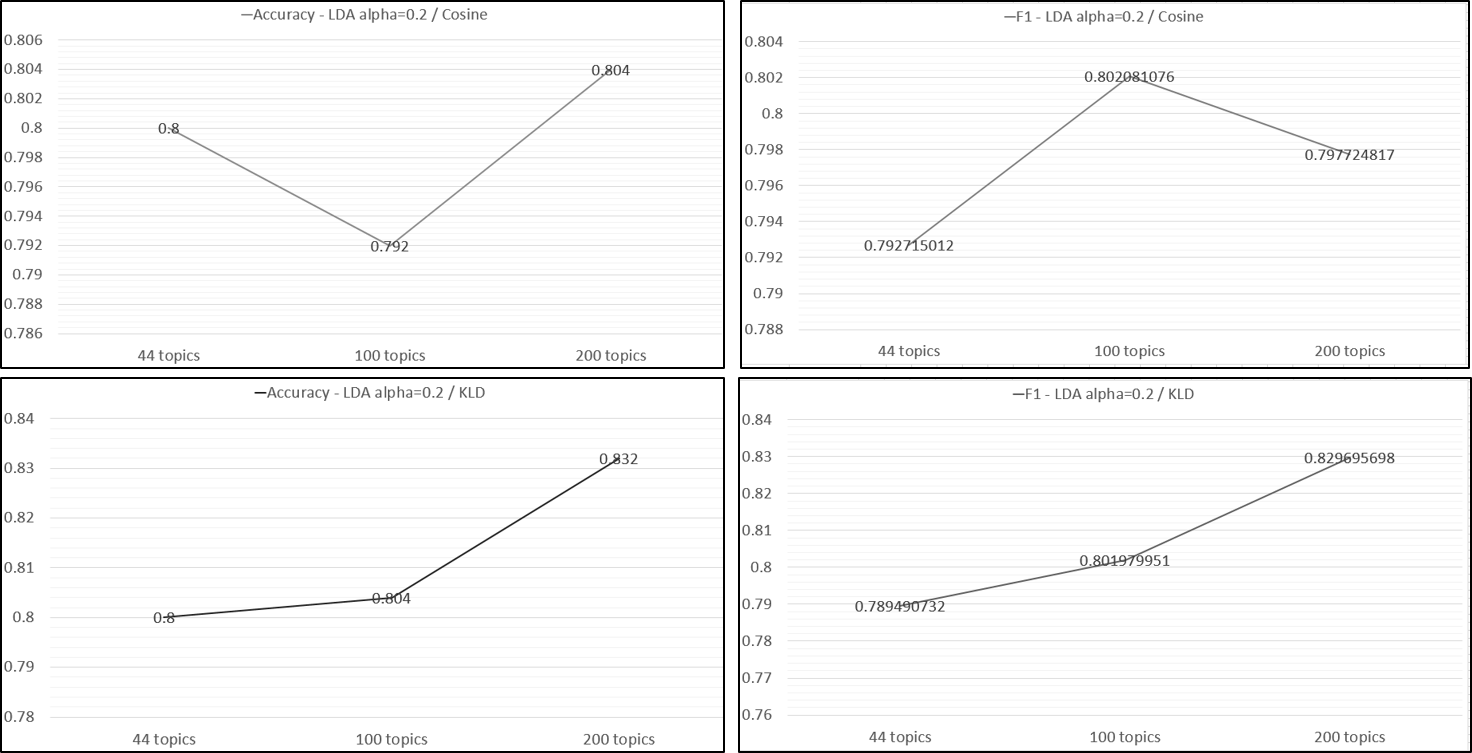
\includegraphics[width=\textwidth]{trend_plot_LDA_more_topics}
\end{figure}


\section{Future work}
\label{future_work}

This work was focused on the analysis of different algorithms intended to work on any text documents dataset. However, as observed in the results of this investigation and other similar works, the solution is strongly dependant on the specific context of the datasets. Based on this, it could be useful to explore the incorporation of more datasets from different sources and analyze the results based on the specific characteristics of each one. A big contribution could consist on applying the studied algorithms to enterprise databases allowing a better understanding of practical applications.\par

Given the importance of data preprocessing on this work, something interesting to evaluate are the different implementations of a same data representation technique. For example, the evaluation of the behavior and the performance of using R versus Python when removing stop words, doing words stemming or TF-IDF weighting.\par

The scope of this investigation was limited to statistical techniques mostly based on lexical analysis of text. A potential good contribution to the experiments could be the incorporation of semantic analysis techniques \cite{seifzadeh2015short,martinez2014analysis,islam2008semantic}, in order to compare the results to the ones obtained in this work.\par 

KNN facilitated the design of experiments because of its simplicity and flexibility to combine data representations and text distance metrics. A future work can consider the use of other supervised classification algorithms and ensemble methods to study their behavior and results respect to KNN.\par

Regarding LDA, there were many aspects left out of the scope of this work but that could represent valuable contributions to the investigation in the future. Firstly, we only used the documents representation generated as part of the model but we didn't apply the complete supervised LDA algorithm. The study and implementation of this algorithm, which doesn't need KNN or text distance metrics, could improve the results by taking advantage of the probabilistic properties of the Dirichlet function and its optimization methods. Second, we can dive deep in optimizing many of the parameters required by LDA to generate the models of topics, looking for a balance between the accuracy of the models and the time it takes to build it. And the third aspect to consider, is the optimization of the existing supervised LDA implementations or to explore alternative topic modelling techniques, looking to improve execution time and lower the complexity.\par

The execution time measurement was not in the scope of this work, but this variable could add an important value to the results, by allowing to clearly identify what are the pros and cons (in terms of performance and eficiency) when using a text distance metric respect to the others.\par

\section{Conclusion}
\label{conclusion}

In this paper we studied different text distance metrics applied to documents classification. These metrics involved text documents representation methods and mathematical functions applied to those representations. We evaluated the accuracy and the F1 score obtained after classifying values using KNN algorithm.\par

The results evidence how the quality of the datasets affected the accuracy and the F1 obtained in all the experiments. For instance, both datasets contained an unbalanced distribution of classes, where one single class covered almos 50\% of the records. We observed a significant improvement in the accuracy after executing the experiments using an hypothetical dataset with balanced classes.\par

LDA achieves an important dimensional reduction as text representation technique, and the experimental results are comparable to the ones achieved by using bag of words, but they were always outperformed by the rest of the studied methods. For both datasets, the number of dimensions in the vectors of topics was up to 150 times smaller than the vectors of words, abstracting thousands of words in less than 60 topics. Some additional experiments suggest that LDA combined with KLD can perform better when used for short text documents, increasing the parameter of number of topics when generating the model and keeping a low value of $\alpha$.\par

\section{Acknowledgements}
\label{acknowledgements}

The authors would like to thank the \textit{Maestr\'{i}a en Computaci\'{o}n} program at \textit{Instituto Tecnol\'{o}gico de Costa Rica} for providing the occasion for this research.

%% The Appendices part is started with the command \appendix;
%% appendix sections are then done as normal sections
%\appendix

%\section{Section in Appendix}
%\label{appendix-sec1}

%Sample text. Sample text. Sample text. Sample text. Sample text. Sample text. 
%Sample text. Sample text. Sample text. Sample text. Sample text. Sample text. 
%Sample text. 

%% References
%%
%% Following citation commands can be used in the body text:
%% Usage of \cite is as follows:
%%   \cite{key}         ==>>  [#]
%%   \cite[chap. 2]{key} ==>> [#, chap. 2]
%%

%% References with bibTeX database:

\bibliographystyle{elsarticle-num}
% \bibliographystyle{elsarticle-harv}
% \bibliographystyle{elsarticle-num-names}
% \bibliographystyle{model1a-num-names}
% \bibliographystyle{model1b-num-names}
% \bibliographystyle{model1c-num-names}
% \bibliographystyle{model1-num-names}
% \bibliographystyle{model2-names}
% \bibliographystyle{model3a-num-names}
% \bibliographystyle{model3-num-names}
% \bibliographystyle{model4-names}
% \bibliographystyle{model5-names}
% \bibliographystyle{model6-num-names}

\bibliography{sample}


\end{document}

%%
%% End of file `elsarticle-template-num.tex'.
